\chapter{Some Big Ideas}

\centering

\includegraphics{images/book-5104342_1920.jpg}

\justifying
There are some key precepts that will serve the aspiring DevSecOps engineer well. In this
chapter we will explore some of these in an attempt to level-set our understanding of the
domain. We will also continue to introduce the reader to the vernacular of the modern day
DevSecOps engineer in a world gone cloudy. You certainly don't need to memorize all of these terms, but the rationale
is they are prevalent enough that you should have a passing familiarity with them, at the very least.

\section{What are DevOps and DevSecOps?}

\justifying
Fundamentally, DevOps and DevSecOps are models for how a team or set of teams can be arranged
to optimize the creation of applications and Infrastructure as Code. They both benefit from
employing similar, if not identical, Agile methodologies. Calling out the ``Security''
piece explicitly in the ``DevSecOps'' nomenclature often signifies an intentional inclusion
of security focused process and activities by the teams involved. Some folks will stick with
the term ``DevOps'', insisting the security piece is still there and just as important, so
there is no need for it to be called out separately.

\justifying
Consider the table \ref{DevSecOps} below. The big takeaway here is to notice the
DevSecOps path goes a bit further
in highlighting security and making it a priority. The goal is to think hard about integrating
security and making it a conscious team effort. Adding a security engineer to DevOps design
and review meetings may not be enough to fuse security into our workflows. We want to ensure
our work products are as secure as possible.

\begin{table}[ht]
    \centering
    \begin{tabular}{|l|c|c|}\hline
                                   & DevOps & DevSecOps \\\hline
        Shifting Left              &   X    &    X       \\\hline
        Automated Security Testing &        &    X       \\\hline
        Policy as Code Testing     &        &    X       \\\hline

    \end{tabular}
\caption{DevOps vs. DevSecOps}
\label{DevSecOps}
\end{table}

\section{Revision Control}

\justifying
Code, documents, test cases, and other software work products begin their lives on the workstations of creators
and developers. In this book we will refer to the environments where this takes place as the ``local'' environment.
These work products are typically created, reviewed and checked into Revision Control Systems
(RCS)\index{Revsion Control System (RCS)}, GitHub\index{GitHub} for example, by the DevSecOps practitioner.
Other popular revision control systems include GitLab\index{GitLab} and BitBucket\index{BitBucket}.

\justifying
Although it may seem like there are a lot of choices when it comes to revision control, there
is one tool that
underlies them all. That tool is known as git. Git is the brainchild of Linus Torvalds, who also
happens to be
the person that invented the Linux kernel just before the turn of the century. This tool work wonderfully
on projects small
and large. For this and may other reasons, it is at the heart of many of these RCS systems that we just mentioned. Note that
in addition to these websites, there are many desktop tools meant to aid developers with revision control on their local
machine. While these can be quite handy, there is no substitute for learning the intricacies of git from the command
line. It will come in quite handy indeed.
\justifying
We will look more closely at git and revision control in a later chapter.

\section{Testing}

\justifying
A test case as a discrete check, or grouping of similar types of checks,
that we use to ensure our work products meet certain minimum standards. Test cases are created with
and often run against our work products at the time they are checked in to the revision control system.
This is meant to ensure stability, security, and compatibility with the existing code base in revision
control. The automation required to execute tests every time work is checked in to
revision control is typically the responsibility of the DevSecOps engineers. We will delve into various
types and aspects of testing throughout this book.

\subsection{White Box vs. Black Box Testing}

\justifying
This is a distinction based on whether you have access to the code, documentation, or hardware under test.
For example, testing the code from a project where you can see the source code would be considered "white box"
testing. You might also look at this as the difference between red\index{Red Team} and blue
teaming\index{Blue Team}. For instance, a "red teamer" or "penetration tester" will typically not have
access to documentation about a system that they are testing.

\section{Pipelines}

\begin{figure}[!htb]
\centering
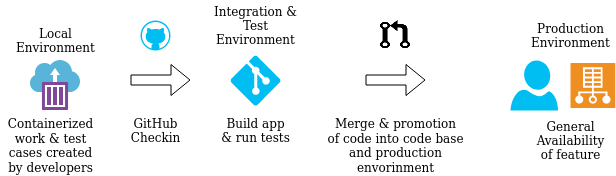
\includegraphics[scale=0.63]{images/flow.png}
\caption{Typical build pipeline}
\label{pipeline}
\end{figure}

\justifying
As seen in figure \ref{pipeline}, work typically flows from the local environments, into a test
environment, and finally to production where it is available for use by the entire user base.

\justifying
We will refer to the entirety of this three-stage flow as one example of what is known as a build pipeline\index{pipeline}.
Code from one or more local environments is checked in to the revision control system throughout a
typical DevSecOps workday, and continuously tested and integrated with the main code base. That is to say, work undergoes
Continuous Integration (CI)\index{Continuous Integration (CI)} with the main code base,
and often Continuous Delivery (CD)\index{Continuous Delivery (CD)} between local, test, and production environments. This is
where the term ``CI/CD Pipeline'' comes from. A business unit may choose to designate more than just the three dev, test,
and prod environments mentioned here, depending on their particular use cases and ways of working.

\justifying
While the CI/CD Pipeline is often a primary focus of the DevSecOps engineer, other pipelines exist as well. For example,
let's assume our organization maintains a vast pool of raw data, also known as a data lake\index{Data Lake}. The staff Data
Engineers build and maintain Data Science\index{Data Science} pipelines to facilitate the smooth flow
of logs and other data into that data lake. Now Data Scientists are able to create machine learning models that rely on that
data to produce useful insights. As another example, consider code changes as they move from
developer workstations into a code repository for storage. Accessing this code for the purpose of testing will differ from
how it is accessed for the purposes of deployment. The order of operations and flow
between differing functions might be said to comprise two different pipelines.

\section{Automation}

\justifying
Consider what may happen when we want to apply the lessons from this book across a large environment made up of many hosts,
containers, pieces of application software, etc. It becomes a huge challenge for an operator to log in to each host or container
individually. Typing, or even cutting and pasting commands to keep things up and running properly, look at logs,
and so on becomes problematic. Creating shell scripts can be quite helpful, but is an outdated modality when we consider
the daunting size and complexity of the modern administrative domain.

\justifying
This is a great use-case for automation. Automation\index{automation} is a way to provision and maintain some or many hosts
in a programmatic manner. Another desirable goal, and hopefully result of automation is to reduce the amount of
per-host interaction that comes with the work of administering systems. Automation is the force multiplier we use to achieve
scaling\index{scaling}. As DevSecOps practitioners, we are on a never-ending quest to achieve
scale-invariance\index{scale-invariance}, to borrow a term from the mathematical realm. That is to say, the tools we
build and processes we engender should work just as well for three machines as they do for three thousand.

\section{Scalability}

\justifying
Bringing together many of the ideas in this section as a foundation, we're able to serve our pipelines and applications from a few users, to many.
Consider the differences between the sort of traffic we can handle with an application on a single server, compared to the
amount of traffic we can handle when we introduce five more servers running the same application code, and a load balancer
to distribute the traffic evenly among these servers.

\justifying
Couple the principle of scalability with the explosive automation tooling ecosystem and you are on the path to doing more,
better work in less time with a smaller staff.

\section{Immutability}

\justifying
There is obvious advantage of being able to quickly stand up new clones of our project to replace existing instances that
may be outdated, insecure, etc. The idea of immutability, in reference to software projects, is the degree to which something,
our running project for example, can be changed. Immutability\index{immutability} is desirable, in that we wish to be able to
simply replace outdated instances of our project in their entirety. Upgrading and patching are inherently
problematic activities, high cost in terms of time, effort and money, that we have the technology to dissociate from. With
containerization, we can more easily achieve immutability across the software life cycle.

\section{Ephemerality}

\justifying
Ephemerality\index{ephemerality} is the concept of something being inherently transitory in nature. For something to be
considered ephemeral, it can exist only briefly. Using immutable containers makes it easier to realize
infrastructure and hosts that are ephemeral. Rather than spending a great deal of time patching and upgrading systems as
we might in a traditional project stack that uses bare metal hosts or even virtual machines, we're going to
use Docker to create a new container in place of the old one. In other words, we're running our project in containers that
are immutable and ephemeral to the degree possible.

\section{GitOps}

\justifying
Just to be sure we have a complete picture of the landscape, we will define the term ``GitOps''\index{GitOps} as a
cloud native analog of Infrastructure as Code being developed with the DevOps/DevSecOps paradigm. Cloud infrastructure
stored in a Git based revision control system can keep a Kubernetes cluster up to date, often with Continuous Deployment.

\section{Organizational Maturity}

\justifying
When I first encounter a new team or group, I try to frame their capabilities in terms of organizational maturity.
Many things can have an effect on the posture of an orgaznization. A few examples:

\begin{itemize}
	\item How many team members there are.
	\item How and how often they interact.
	\item  What productivity tools do they use?
	\item How often and Why do they meet?
	\item How their work is captured, completed, and reviewed?
\end{itemize}

The structure of a team and the tendency to follow best practices, as well as their own policies, tend to provide some
valuable insight. The measure of these insights is the maturity of the team. Even a cursory and informal aanalysis can give
a sense of challenges that might arise during creation of work products in terms of time, potential quality, and of course,
the security of any output. The importance of the maturiy of an organization stems from it's high degree to which it shapes
the effectiveness of that organization.

\justifying
Let's consider Conway's Law:

\begin{displayquote}
    \emph{Any organization that designs a system (defined broadly) will produce a design whose structure is a copy of the
organization's communication structure.}

Melvin E. Conway
\end{displayquote}

\justifying
As with so many things in life, communication is a fundamental key to team success. Keep in mind that each DevSecOps
team is somewhere on the spectrum in terms of their capability and organizational maturity, whether they realize it or not!
There is a direct correlation between the maturity of the team and the results you will get from them. Of course there are
plenty of decent blogs and articles on the web that provide detail on the ``DevSecOps Maturity Model'' in case you want to
dig deeper on this subject.
